\section{Conics in Polar Coordinates}\label{sec:Conics in Polar Coordinates}
A \dfont{conic section}\index{conic section}\index{polar coordinates!conic section} is a curve obtained as the intersection of a 
cone and a plane. One useful geometric definition that only involves the plane
is that a conic consists of those points whose distances to some point, called a 
\dfont{focus}, and some line, called a \dfont{directrix}, are in a fixed ratio, 
called the \dfont{eccentricity}.

The three types of conic sections are the ellipse, parabola and hyperbola (with the circle being a degenerate case of an ellipse).

$$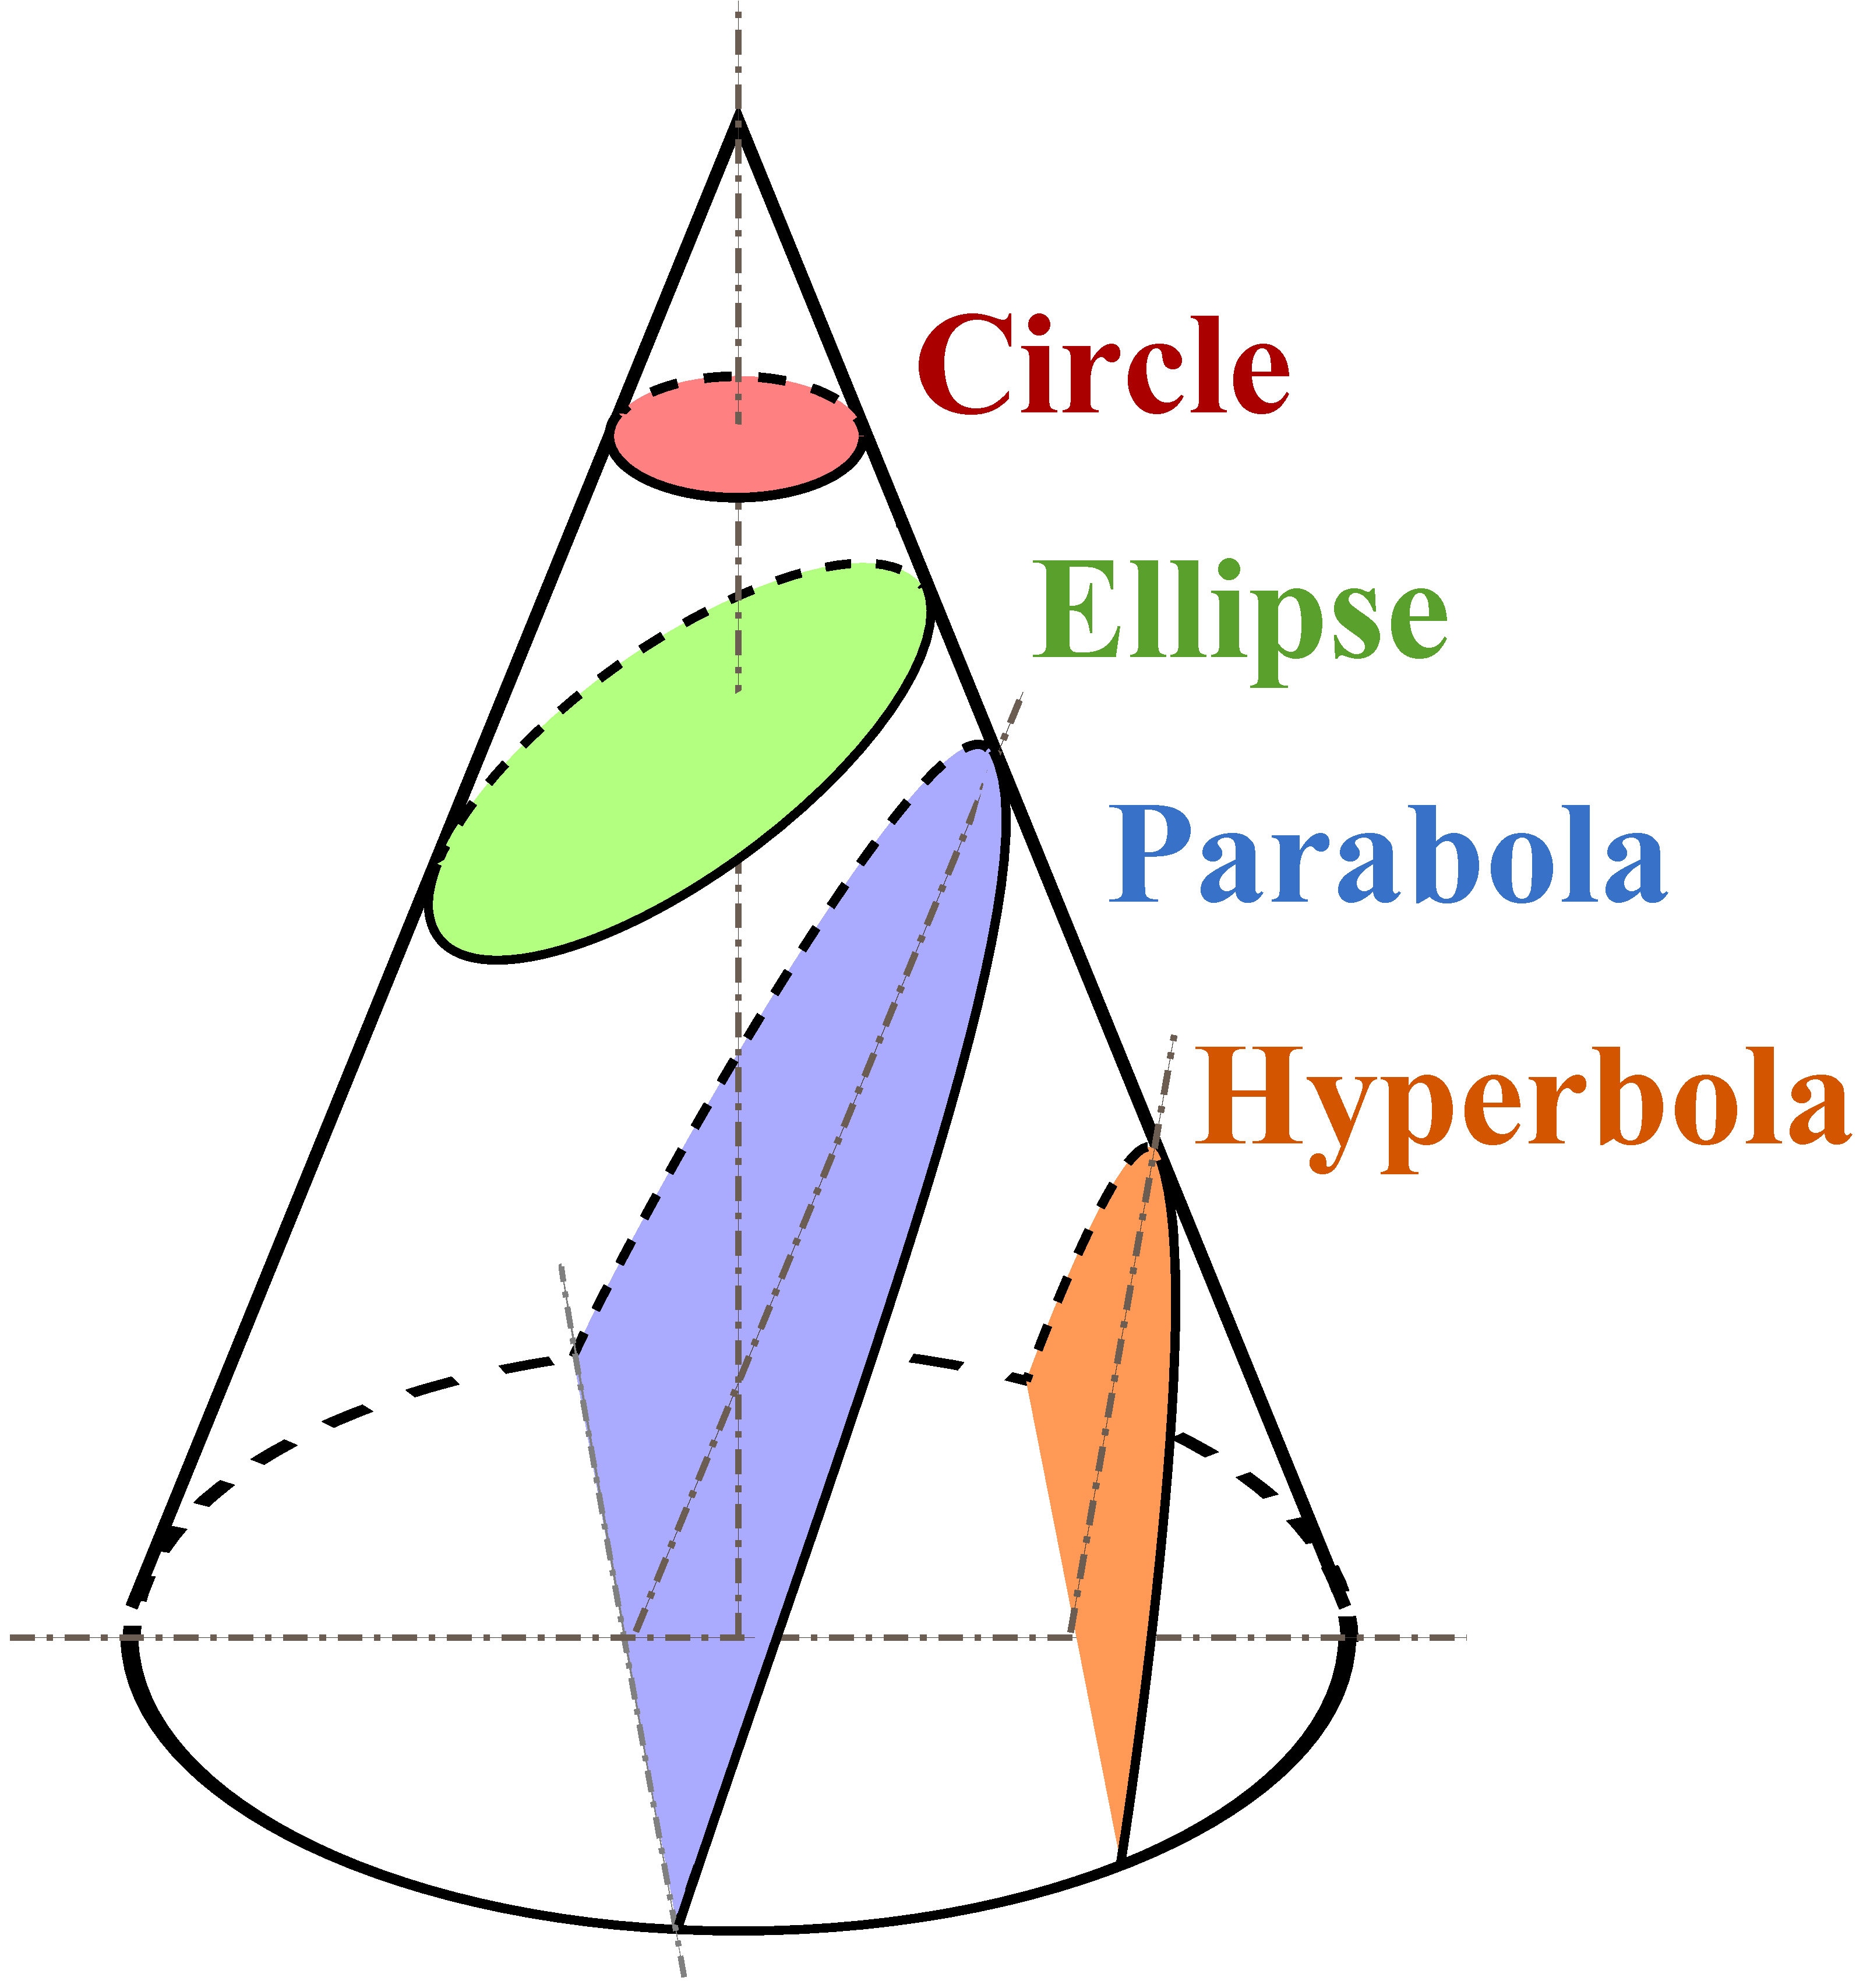
\includegraphics[width=3in]{images/ConicSections}$$

Let $F$ be a fixed point (the focus), $L$ be a line (the directrix) not containing $F$ and $e$ be a nonnegative real number (the eccentricity).
The conics sections are obtained by the set of all points $P$ whose distance to $F$ equals $e$ times their distance to $L$, that is:
$$\frac{|PF|}{|PL|}=e.$$
In the case that:
\begin{itemize}\setlength{\itemsep}{0 in}
\item $e<1$ we obtain an ellipse (and when $e=0$ we obtain the degenerate case: A circle),
\item $e=1$ we obtain a parabola,
\item $e>1$ we obtain a hyperbola.
\end{itemize}

To obtain a simple polar equation we place the focal point at the origin.
The formulation for a conic section is then given in the polar form by
$$r=\frac{pe}{1\pm e\cos\theta}\qquad\mbox{and}\qquad r=\frac{pe}{1\pm e\sin\theta}$$
where $e$ is the eccentricity and $p$ is the focal parameter representing the distance from the focus (or one of the two foci) to the directrix.

The three different types of conic sections are shown below. Focal points corresponding to all conic sections are placed at the origin.
First is the parabola.
$$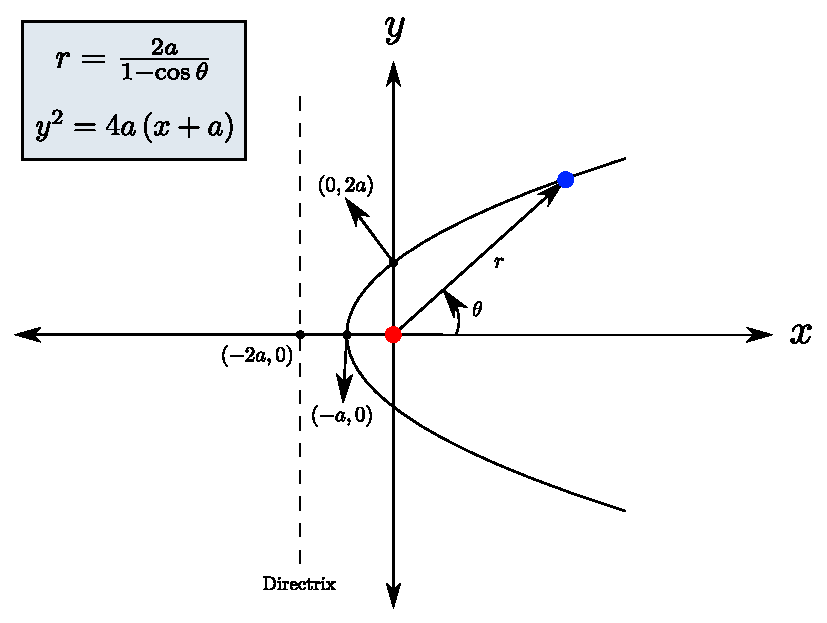
\includegraphics[width=5in]{images/conics-polar1}$$
Next is the ellipse.
$$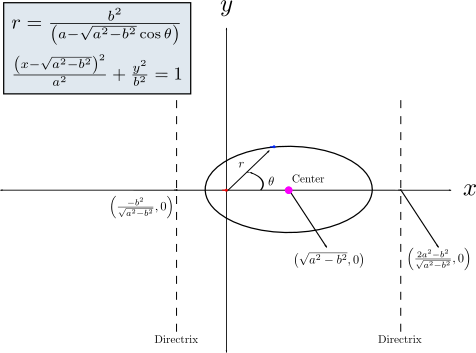
\includegraphics[width=5in]{images/conics-polar2}$$
Finally, we have the hyperbola.
$$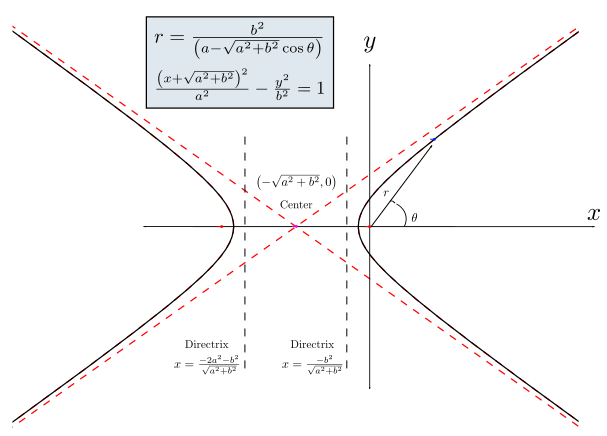
\includegraphics[width=5in]{images/conics-polar3}$$

Some things to keep in mind with respect to the denominator of polar equations of various conics are the following:
\begin{itemize}\setlength{\itemsep}{0 in}
\item If the denominator is $1 + e \sin\theta$, it has a horizontal directrix above the focal point.
\item If the denominator is $1 - e \sin\theta$, it has a horizontal directrix below the focal point.
\item If the denominator is $1 + e \cos\theta$, it has a vertical directrix to the right of the focal point.
\item If the denominator is $1 - e \cos\theta$, it has a vertical directrix to the left of the focal point. 
\end{itemize}

\begin{example}{Polar Equations for a Parabola}{polareqnparabola}
Find the equation of a parabola with focus at the origin and whose directrix is the line $x=-1$.
\end{example}

\begin{solution}
Since we have a parabola, $e=1$.
Furthermore, $p=1$.
Since the graph has a vertical directrix, the equation will use $1 - e \cos\theta$ in the denominator.
Thus, the equation is:
$$r=\frac{2}{1-\sin\theta}$$
\end{solution}


%%%%%%%%%%%%%%%%%%%%%%%%%%%%%%%%%%%%%%%%%%%%
\Opensolutionfile{solutions}[ex]
\section*{Exercises for \ref{sec:Conics in Polar Coordinates}}

\begin{enumialphparenastyle}

%%%%%%%%%%
\begin{ex}
\noindent Identify the following conics and find the eccentricity.
\begin{multicols}{2}
\begin{enumerate}
	\item	$\ds r=\frac{2}{1+\sin\theta}$
	\item	$\ds r=\frac{4}{2+\cos\theta}$
	\item	$\ds r=\frac{3}{1-\sin\theta}$
	\item	$\ds r=\frac{5}{2+2\sin\theta}$
\end{enumerate}
\end{multicols}
\end{ex}


%%%%%%%%%%
\begin{ex}
Write the polar equation of a parabola with focus at the origin and directrix $x=3$.
\end{ex}

%%%%%%%%%%
\begin{ex}
Write the polar equation of a hyperbola with focus at the origin, directrix $x=4$ and eccentricity $2$.
\end{ex}

%%%%%%%%%%
\begin{ex}
Write the polar equation of an ellipse with focus at the origin, directrix $x=4\sec\theta$ and eccentricity $1/2$.
\end{ex}

\end{enumialphparenastyle}
